\documentclass{article}
\usepackage[legalpaper, margin=1in]{geometry}
\usepackage[utf8]{inputenc}
\usepackage{hyperref}
\usepackage{graphicx}
\usepackage{float}
\usepackage{listings}
\usepackage{minted}
\usepackage{xcolor}
\usepackage{caption}
\definecolor{LightGray}{gray}{0.9}
\setminted{
	linenos=true,
	autogobble,
}
% Create a new environment for breaking code listings across pages.
\newenvironment{longlisting}{\captionsetup{type=listing}}{}

\title{\underline{\textbf{MoTiVML Guideline Document}}}
\author{}
\date{}

\begin{document}

\maketitle
\textit{This is a guideline document for the MoTiVML language and framework as a whole. This guideline document assists end users in modelling variability in robotic systems as well as implementing the features they have defined in their models. As a supporting artifact to the language,  this document serves as a form of verification for the MoTiVML language and its capabilities.}

\noindent\rule{17cm}{0.4pt}

\label{guide:docs}
\section{Prerequisites and Dependencies}
    \begin{itemize}
        \item Ubuntu 20.04.3 LTS and above
        \item ROS installation. This application was developed and tested with ROS Neotic 1.15.9.
        \item Python3 installation
        \item C++ 11 or higher
        \item ROS Pluginlib
    \end{itemize}

\section{Framework Components}
\begin{itemize}
	\item Domain Specific Language
	\item Modeller
	\item Configurator
	\item Model visualizer
	\item Syntax and Semantics Validator
	\item Feature Plugin Interface
\end{itemize}

\section{Setup and Installation of MoTiVML}
\begin{itemize}
    \item Clone MoTiVML from \href{https://github.com/SergioGarG/sera-extension}{here} into your catkin workspace.
    \item Go the MoTiVML workspace project directory and build the cloned project with the command catkin\_make and press enter on your keyboard.
\end{itemize}

\section{How To}
This section gives a step-by-step walk-through of how MoTiVML can be used to instantiate a model or configuration, how it can be used to validate a model as well as the capability to link source code implementations with feature definitions. We also give a brief tutorial of our in-built MoTiVML console interface. Throughout our demonstrations in this guideline document, we use a sample model of a robotic system that is shown graphically in figure \ref{simplebot}. This graphical representation of a simple robot model will also serve as our running example throughout this document.

\begin{figure}[H]
	\caption{Graphical Model of a Simple Robot}
	\centering
	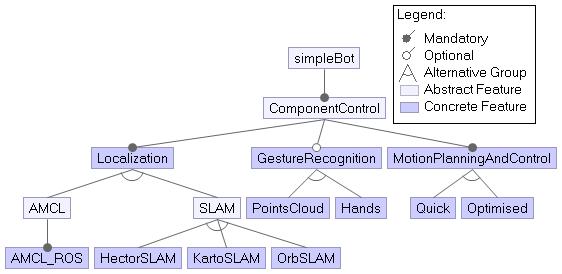
\includegraphics[width=\columnwidth]{images/simpleBot.png}
	\label{simplebot}
\end{figure}

\subsection{Instantiate a MoTiVML Model}
\begin{itemize}
	\item To create an instance of a model in MoTiVML, in the \textbf{src} folder of the cloned application, make a copy of the template folder provided and rename it to suit your product preference.
	
	\item In your new product instance folder, there is a \textbf{model.json} with an existing root feature, wrapped in a object.
	
	\item The model definition can be extended by appending sub features to the root feature. You can add nested feature objects according to your preferences.Note that each feature specification must have attributes such as \textbf{id}, \textbf{name}, \textbf{constraints}, \textbf{group}, \textbf{isMandatory}. The constraints attribute must contain sub attributes \textbf{featureIncluded}, \textbf{featureExcluded}, \textbf{bindingTimeAllowed}, \textbf{bindingModeAllowed}. Listing \ref{feat-schema} shows a demonstrated example of an extended MoTiVML model instance, for the feature model captured in Figure \ref{simplebot}.
	
	\item The value of each feature attribute in a model must conform to strict type systems defined within MoTiVML. A list of all the attributes together with their expected values is provided below in Table \ref{tab:valueTypes}.
	
	\begin{table}[H]
		\caption{Feature Attributes and Types}
			\begin{tabular}{|l|p{10cm}|}
				\hline
				Attribute & Expected Value \\\hline
				id & Alphanumeric characters. No spaces allowed.   \\ \hline
				name & Alphanumeric characters. No spaces allowed.   \\ \hline
				constraints & Object containing attributes \textbf{featureIncluded}, \textbf{featureExcluded}, \textbf{bindingTimeAllowed}, \textbf{bindingModeAllowed}  \\ \hline
				featureIncluded & Array of existing feature "ids" \\ \hline
				
				featureExcluded & Array of existing feature "ids" \\ \hline
				bindingTimeAllowed & Early / Late / Any \\ \hline
				bindingModeAllowed & Static / Dynamic / Any \\ \hline
				
				group & XOR / OR \\ \hline
				isMandatory & True or False \\ \hline
				
			\end{tabular}
			\label{tab:valueTypes}
	\end{table}
	
	\item To add a sub-feature to a defined feature, add the \textbf{sub} attribute to the feature and assign an array of sub-feature objects to it. However, the sub attribute is optional. Features that do not have sub-features can exist without a \textbf{sub} attribute.
	
\end{itemize}


\begin{longlisting}
	\caption{SimpleRobot Model Instantiation in MoTiVML}
	\begin{minted}[
		framesep=1mm,
		baselinestretch=1.2,
		bgcolor=LightGray,
		fontsize=\footnotesize
		]{Json}
		
		{
			"id": "root_feature",
			"name": "SimpleBot",
			"group": "",
			"isMandatory": true,
			"isSelected": true,
			"sub": [
			{
				"id": "compcontrol",
				"name": "ComponentControl",
				"constraints": {
					"featuresIncluded": [],
					"featuresExcluded": [],
					"bindingTimeAllowed":"Early",
					"bindingModeAllowed":"Static"
				},
				"group": "OR",
				"isMandatory": true,
				"sub":[
				{
					"id": "localztn",
					"name": "Localisation",
					"constraints": {
						"featuresIncluded": [],
						"featuresExcluded": [],
						"bindingTimeAllowed":"Early",
						"bindingModeAllowed":"Static"
					},
					"group": "OR",
					"isMandatory": true,
					"sub":[
					{
						"id": "amcl",
						"name": "AMCL",
						"constraints": {
							"featuresIncluded": [],
							"featuresExcluded": [],
							"bindingTimeAllowed":"Early",
							"bindingModeAllowed":"Static"
						},
						"group": "XOR",
						"isMandatory": false,
						"sub":[
						{
							"id": "amclros",
							"name": "AmclRos",
							"constraints": {
								"featuresIncluded": [],
								"featuresExcluded": [],
								"bindingTimeAllowed":"Early",
								"bindingModeAllowed":"Static"
							},
							"group": "OR",
							"isMandatory": true
						}
						]
					},
					{
						"id": "slam",
						"name": "SLAM",
						"constraints": {
							"featuresIncluded": [],
							"featuresExcluded": [],
							"bindingTimeAllowed":"Early",
							"bindingModeAllowed":"Static"
						},
						"group": "XOR",
						"isMandatory": false,
						"sub":[
						{
							"id": "hectorslam",
							"name": "HectorSLAM",
							"constraints": {
								"featuresIncluded": [],
								"featuresExcluded": ["kartoslam", "orbslam"],
								"bindingTimeAllowed":"Late",
								"bindingModeAllowed":"Dynamic"
							},
							"group": "XOR",
							"isMandatory": false
						},
						{
							"id": "kartoslam",
							"name": "KartoSLAM",
							"constraints": {
								"featuresIncluded": [],
								"featuresExcluded": ["orbslam", "hectorslam"],
								"bindingTimeAllowed":"Late",
								"bindingModeAllowed":"Dynamic"
							},
							"group": "XOR",
							"isMandatory": false
						},
						{
							"id": "orbslam",
							"name": "OrbSLAM",
							"constraints": {
								"featuresIncluded": [],
								"featuresExcluded": ["kartoslam", "hectorslam"],
								"bindingTimeAllowed":"Late",
								"bindingModeAllowed":"Dynamic"
							},
							"group": "XOR",
							"isMandatory": false
						}
						]
					}
					]
				},
				{
					"id": "gestrec",
					"name": "GestureRecognition",
					"constraints": {
						"featuresIncluded": [],
						"featuresExcluded": [],
						"bindingTimeAllowed":"Early",
						"bindingModeAllowed":"Static"
					},
					"group": "OR",
					"isMandatory": false,
					"sub":[
					{
						"id": "hands",
						"name": "Hands",
						"constraints": {
							"featuresIncluded": [],
							"featuresExcluded": ["pointscloud"],
							"bindingTimeAllowed":"Late",
							"bindingModeAllowed":"Dynamic"
						},
						"group": "XOR",
						"isMandatory": false
					},
					{
						"id": "pointscloud",
						"name": "PointsCloud",
						"constraints": {
							"featuresIncluded": [],
							"featuresExcluded": ["hands"],
							"bindingTimeAllowed":"Late",
							"bindingModeAllowed":"Dynamic"
						},
						"group": "XOR",
						"isMandatory": false
					}
					]
				},
				{
					"id": "motplannctrl",
					"name": "MotionPlanningAndControl",
					"constraints": {
						"featuresIncluded": [],
						"featuresExcluded": [],
						"bindingTimeAllowed":"Early",
						"bindingModeAllowed":"Static"
					},
					"group": "OR",
					"isMandatory": true,
					"sub":[
					{
						"id": "quick",
						"name": "Quick",
						"constraints": {
							"featuresIncluded": [],
							"featuresExcluded": ["optimised"],
							"bindingTimeAllowed":"Late",
							"bindingModeAllowed":"Dynamic"
						},
						"group": "XOR",
						"isMandatory": false
					},
					{
						"id": "optimised",
						"name": "Optimised",
						"constraints": {
							"featuresIncluded": [],
							"featuresExcluded": ["quick"],
							"bindingTimeAllowed":"Late",
							"bindingModeAllowed":"Dynamic"
						},
						"group": "XOR",
						"isMandatory": false
					}
					]
				}
				]
			}
			]
		}
		
	\end{minted}
	\label{feat-schema}
\end{longlisting}

\subsection{Instantiate a MoTiVML Configuration}

\begin{itemize}
	\item Again in your instance folder, there is a \textbf{config.json} with an empty \textbf{properties} array value.
	
	\item In the config.json file of your project, for every feature added in your model.json file, a corresponding configuration object must be added. For each feature configuration object, there must be an \textbf{id} attribute which references the \textbf{id} of a feature in your model.json file. The \textbf{props} attribute must contain \textbf{time} and \textbf{mode} attributes.  Listing \ref{conf-schema} shows a MoTiVML configuration translation of the features present in Figure \ref{simplebot}.
	
	\item The values of each configuration attribute for your model must conform to strict type systems defined within MoTiVML. A list of all the configuration attributes together with their expected values is provided below in Table \ref{tab:confvalueTypes}.
	
	\begin{table}[H]
		\caption{Configuration Attributes and Types}
		\begin{tabular}{|l|p{10cm}|}
			\hline
			Attribute & Expected Value \\\hline
			id & Alphanumeric characters. No spaces allowed.   \\ \hline
			props & Object containing attributes \textbf{time} and \textbf{mode} \\ \hline
			time & Early / Late  \\ \hline
			mode & Static / Dynamic \\ \hline
		\end{tabular}
		\label{tab:confvalueTypes}
	\end{table}
	
\end{itemize}

\begin{longlisting}
	\caption{SimpleRobot Model Configuration Instantiation in MoTiVML}
	\begin{minted}[
		framesep=2mm,
		baselinestretch=1,
		bgcolor=LightGray,
		fontsize=\footnotesize
		]{Json}
		
		{
			"properties": [
			{
				"id": "compcontrol",
				"props": {
					"time":"Early",
					"mode":"Static"
				}
			},
			{
				"id": "localztn",
				"props": {
					"time":"Early",
					"mode":"Static"
				}
			},
			{
				"id": "gestrec",
				"props": {
					"time":"Early",
					"mode":"Static"
				}
			},
			{
				"id": "motplannctrl",
				"props": {
					"time":"Early",
					"mode":"Static"
				}
			},
			{
				"id": "amcl",
				"props": {
					"time":"Early",
					"mode":"Static"
				}
			},
			{
				"id": "amclros",
				"props": {
					"time":"Early",
					"mode":"Static"
				}
			},
			{
				"id": "slam",
				"props": {
					"time":"Early",
					"mode":"Static"
				}
			},
			{
				"id": "hectorslam",
				"props": {
					"time":"Late",
					"mode":"Dynamic"
				}
			},
			{
				"id": "kartoslam",
				"props": {
					"time":"Late",
					"mode":"Dynamic"
				}
			},
			{
				"id": "orbslam",
				"props": {
					"time":"Late",
					"mode":"Dynamic"
				}
			},
			{
				"id": "hands",
				"props": {
					"time":"late",
					"mode":"Dynamic"
				}
			},
			{
				"id": "pointscloud",
				"props": {
					"time":"Late",
					"mode":"Dynamic"
				}
			},
			{
				"id": "quick",
				"props": {
					"time":"Late",
					"mode":"Dynamic"
				}
			},
			{
				"id": "optimised",
				"props": {
					"time":"Late",
					"mode":"Dynamic"
				}
			}
			]
		}
	\end{minted}
	\label{conf-schema}
\end{longlisting}

\subsection{Use the Standalone Model Validator Tool}
The inbuilt motivml model validator tool aids in validating models together with their corresponding configurations. To validate your model and its configuration, navigate to the \textbf{/src/motivml} directory and run the following command in the ROS console:

\begin{longlisting}
	\caption{MoTiVML Validation Command}
	\begin{minted}[
		framesep=2mm,
		baselinestretch=1,
		bgcolor=LightGray,
		fontsize=\footnotesize
		]{python}
		
		python validator.py <project_directory_name>

	\end{minted}
\label{valcomm}
\end{longlisting}

All models created in the MoTiVML language are validated on two distinct levels. i.e. syntactically and semantically. Syntactical validation has to do with feature and configuration schemas being evaluated for errors, while semantic validation has to do with modelling and binding constraints evaluation.

To demonstrate this we evaluate our constructed model and configuration shown in Listing \ref{feat-schema} and \ref{conf-schema} and discuss the results accordingly. A careful observation of  the console output generated from the validation indicates the presence of zero errors. 

When our in-built schema and constraint checker identify an error in either a model or a configuration, an error message is outputted to the console indicating where the error is located and why the language has flagged it as an error.

\begin{figure}[H]
	\caption{Simplebot Validation Output}
	\centering
	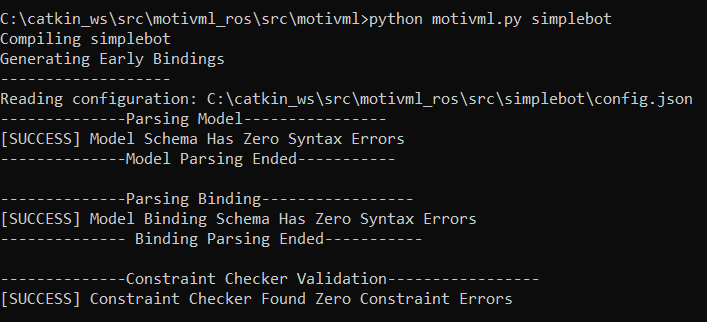
\includegraphics[width=\columnwidth]{images/validate.png}
	\label{validation}
\end{figure}

%%Upon successfully validating a model without any errors, a \textbf{bindings.motivml} file is generated in the corresponding project folder. This file contains features that are have been bound at compile time. At runtime, the \textbf{bindings.motivml} file is dynamically updated depending on which features are successfully bound or unbound.

\subsection{Implement a Statically Bound Feature}
\subsubsection{Static Early}
\begin{itemize}
	\item In the \textbf{featx} directory, create a static class in the namespace \textbf{static\_integration} which inherits from the class \textbf{public static\_base::StaticInterface}. NB: The feature id in your model must match your class name. For Example:
	
	\begin{longlisting}
		\caption{Sample Static Early Class}
		\begin{minted}[
			framesep=2mm,
			baselinestretch=1.2,
			bgcolor=LightGray,
			fontsize=\footnotesize
			]{C}
			
			namespace static_integration{
				
				class MyStaticEarlyClass: public static_base::StaticInterface{
					std::string feature_id = "my_unique_feature_id";
					public:
					MyStaticEarlyClass(){};
					
					void executeFeature(){
						std::cout << "Hello My Feature!!" << std::endl;
					};
					
				};
				
			};
			
		\end{minted}
		\label{samplestaticearly}
	\end{longlisting}
	\item Set the class variable \textbf{feature\_id} to the same value as the \textbf{id} attribute in the MoTiVML model.
	\item Add the following preprocessor include above your class to include the static base interface class your class will be inheriting from:
	\begin{longlisting}
		\caption{Class Inclusion}
		\begin{minted}[
			framesep=2mm,
			baselinestretch=1.2,
			bgcolor=LightGray,
			fontsize=\footnotesize
			]{C}
			
			#include "../include/motivml_ros/static_base.h"
			
		\end{minted}
		\label{classinclude}
	\end{longlisting}
	\item Define a static early feature constant at the top of \textbf{plugin\_feature\_loader.cpp}. For Example
	
	\begin{longlisting}
		\caption{Constant Definition}
		\begin{minted}[
			framesep=2mm,
			baselinestretch=1.2,
			bgcolor=LightGray,
			fontsize=\footnotesize
			]{C}
			
			#define UNKOWNFEATURE
			
		\end{minted}
		\label{definepreproccomm}
	\end{longlisting}
	
	\item In \textbf{static\_feature\_loader.h}, if the feature constant you created in the previous step is true, include your static class. See Listing \ref{includestatclass} as an example
	\begin{longlisting}
		\caption{Including Static Early}
		\begin{minted}[
			framesep=2mm,
			baselinestretch=1.2,
			bgcolor=LightGray,
			fontsize=\footnotesize
			]{C}
			
			#ifdef UNKOWNFEATURE
			#include "../../featx/MyStaticClass.h"
			#endif
			
		\end{minted}
		\label{includestatclass}
	\end{longlisting}

	\item Extent the static early conditional block of the \textbf{callback\_load\_plugin\_features} method in \textbf{plugin\_feature\_loader.cpp} to run a method in your static early class.
	
	\item Run the \textbf{catkin\_make} command to build the project.
\end{itemize}

\subsubsection{Static Late}
%% pluginlib steps with alteration guard
\begin{itemize}
	\item In the \textbf{featx} directory, create a static class in the namespace \textbf{static\_integration} which inherits from the class \textbf{public static\_base::StaticInterface}. NB: The feature id in your model must match your class name. For Example:
	
	\begin{longlisting}
		\caption{Sample Static Late Class}
		\begin{minted}[
			framesep=2mm,
			baselinestretch=1.2,
			bgcolor=LightGray,
			fontsize=\footnotesize
			]{C}
			
			namespace static_integration{
				
				class MyStaticLateClass: public static_base::StaticInterface{
					std::string feature_id = "my_unique_feature_id";
					public:
					MyStaticEarlyClass(){};
					
					void executeFeature(){
						std::cout << "Hello My Feature!!" << std::endl;
					};
					
				};
				
			};
			
		\end{minted}
		\label{samplestaticlate}
	\end{longlisting}
	\item Statically include the feature in the configuration by adding it to the \textbf{motivml\_plugins.h} file. For Example
	
	\begin{longlisting}
		\caption{Sample Static Late Class}
		\begin{minted}[
			framesep=2mm,
			baselinestretch=1.2,
			bgcolor=LightGray,
			fontsize=\footnotesize
			]{C}
			
			#include "../../featx/MyStaticLateClass.h"
			
		\end{minted}
		\label{samplestaticlateinclude}
	\end{longlisting}
	
	\item To get the feature to be loaded at runtime, use pluginlib to export your class to the static interface. For example 
	
	\begin{longlisting}
		\caption{Sample Static Late Class}
		\begin{minted}[
			framesep=2mm,
			baselinestretch=1.2,
			bgcolor=LightGray,
			fontsize=\footnotesize
			]{C}
			
			PLUGINLIB_EXPORT_CLASS(static_integration::MyStaticLateClass, static_base::StaticInterface)
			
		\end{minted}
		\label{pluginexport}
	\end{longlisting}
	
	\item Provide meta-date about your static late feature to pluginlib, by registering the exported class in the  \textbf{motivml\_plugins.xml} file stating the class name and description of your class. For example
	
	\begin{longlisting}
		\caption{Sample Static Late Class}
		\begin{minted}[
			framesep=2mm,
			baselinestretch=1.2,
			bgcolor=LightGray,
			fontsize=\footnotesize
			]{xml}
			
			<class type="static_integration::MyStaticLateClass" base_class_type="static_base::StaticInterface">
				<description>Description of class goes here</description>
			</class>
			
		\end{minted}
		\label{samplestaticlatedesc}
	\end{longlisting}
	
\end{itemize}

\subsection{Implement a Dynamically Bound Feature}
\begin{itemize}
	\item In the \textbf{featx} directory, create a static class in the namespace \textbf{static\_integration} which inherits from the class \textbf{public static\_base::StaticInterface}. NB: The feature id in your model must match your class name. For Example:
	
	\begin{longlisting}
		\caption{Sample Dynamic Class}
		\begin{minted}[
			framesep=2mm,
			baselinestretch=1.2,
			bgcolor=LightGray,
			fontsize=\footnotesize
			]{C}
			
			namespace motivml_plugins{
				
				class MyDynamicClass: public plugin_base::PluginInterface{
					std::string feature_id = "my_unique_feature_id";
					public:
					MyDynamicClass(){};
					
					void executeFeature(){
						std::cout << "Hello My Feature!!" << std::endl;
					};
					
				};
				
			};
			
		\end{minted}
		\label{samplestaticlate}
	\end{longlisting}

	\item \textbf{Include Plugin}: Include the feature in the configuration by adding it to the \textbf{motivml\_plugins.h} file. For Example
	
	\begin{longlisting}
		\caption{Sample Static Late Class}
		\begin{minted}[
			framesep=2mm,
			baselinestretch=1.2,
			bgcolor=LightGray,
			fontsize=\footnotesize
			]{C}
			
			#include "../../featx/MyDynamicClass.h"
			
		\end{minted}
		\label{sampstaticlateinclude}
	\end{longlisting}

	\item \textbf{Encapsulate Feature As Plugin}: In order to allow a class to be dynamically loaded, it must be marked as an exported class. This is done through the special macro PLUGINLIB\_EXPORT\_CLASS  \cite{pluginlib}. For example
	
	\begin{longlisting}
		\caption{Sample Dynamic Class Export}
		\begin{minted}[
			framesep=2mm,
			baselinestretch=1.2,
			bgcolor=LightGray,
			fontsize=\footnotesize
			]{C}
			
			PLUGINLIB_EXPORT_CLASS(motivml_plugins::MyDynamicClass, plugin_base::PluginInterface)
			
		\end{minted}
		\label{pluginexport}
	\end{longlisting}
	
	\item \textbf{Add Plugin Description: } The plugin description file is an XML file that serves to store all the important information about a plugin in a machine readable format. It contains information about the library the plugin is in, the name of the plugin, the type of the plugin, etc \cite{pluginlib}. Ihe plugin description file (motivml\_plugin.xml), would look something like this:
	
	\begin{longlisting}
		\caption{Sample Static Late Class}
		\begin{minted}[
			framesep=2mm,
			baselinestretch=1.2,
			bgcolor=LightGray,
			fontsize=\footnotesize
			]{xml}
			
			<class type="motivml_plugins::MyDynamicClass" base_class_type="plugin_base::PluginInterface">
				<description>Description of class goes here</description>
			</class>
			
		\end{minted}
		\label{sampledylatedesc}
	\end{longlisting}
	
\end{itemize}



\subsection{MoTiVML Console Interface}
To add some interactivity to our variability modelling language, we have provided an in-built console interface for interacting with models and features through MoTiVML specific commands.

To launch the MoTiVML console interface, navigate to the \textbf{/src/motivml} directory and run the following command in Listing \ref{console}:

\begin{longlisting}
	\caption{MoTiVML Console Launch Command}
	\begin{minted}[
		framesep=2mm,
		baselinestretch=1.2,
		bgcolor=LightGray,
		fontsize=\footnotesize
		]{python}
		
		python mmconsole.py <project_directory_name>
		
	\end{minted}
	\label{console}
\end{longlisting}

When the above command is run, the model and configuration defined in the \textbf{project\_directory\_name} is compiled and validated, prior to the console interface being launched. If there are no errors detected, the console interface is then launched successfully. 

\begin{figure}[H]
	\caption{Simplebot Console}
	\centering
	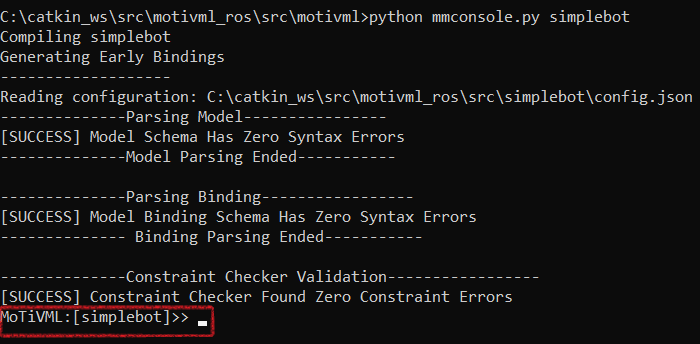
\includegraphics[width=\columnwidth]{images/console.png}
	\label{consolelaunch}
\end{figure}

In Figure \ref{consolelaunch} we can observe the launched MoTiVML console. As highlighted in the figure above, the console prompt always bears the name of the project which was launched with the console. For this reason, all MoTiVML console commands that are run will be affiliated with the model highlighted in the console prompt.

\subsection{MoTiVML Console Commands}
\begin{itemize}
	\item \textbf{show $<parameter>$}: The show command invokes the motivml model visualizer. The show command is used to display graphically a user constructed model. This command prints the hierarchical structure of a selected model while displaying details such as its mandatory status, group and binding mode. The show command takes a single parameter. This parameter can either be \textbf{all} or  \textbf{config}. \\
	
	The \textbf{show all} command only visualizes all selected features that exist in a model tree. By default all features are selected when instantiated. Thus, this command shows every single feature in the model tree.
	
	\begin{figure}[H]
		\caption{show all Command}
		\centering
		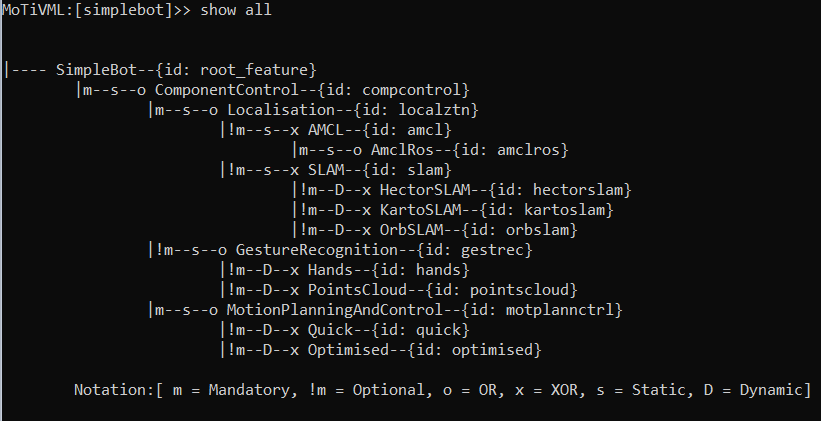
\includegraphics[width=\columnwidth]{images/showall.png}
		\label{showall}
	\end{figure}

	The \textbf{show config} command only visualizes currently selected or bound features. That is, unselected or unbound features in the model are excluded from the visualizer output.

	\begin{figure}[H]
		\caption{show config Command}
		\centering
		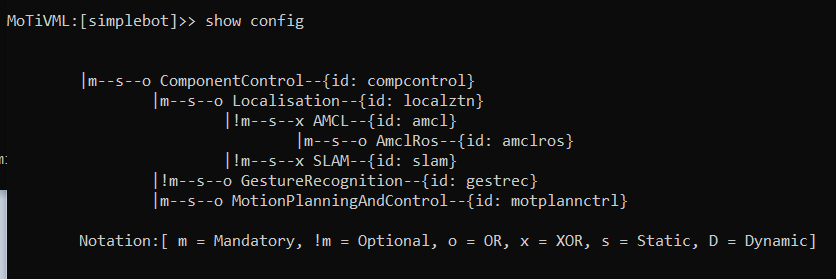
\includegraphics[width=\columnwidth]{images/showconfig.png}
		\label{showconfig}
	\end{figure}
	
	\item \textbf{exit}: The exit command shuts down the console interface and returns back to the original ROS console. The exit command also asks for a yes or no confirmation before proceeding. Figure \ref{exit} shows an exit command execution and output.
	\begin{figure}[H]
		\caption{Exit Command}
		\centering
		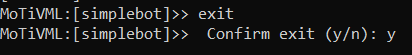
\includegraphics[width=8cm]{images/exit.png}
		\label{exit}
	\end{figure}

	\item \textbf{load $<feature id>$}: The load command attempts to add a feature to the existing configuration. Once the feature is added successfully to the configuration, the feature is executed to show its existence.
	
	\item \textbf{unload $<feature id>$}:The unload command attempts to remove a feature from the existing configuration. Once the feature is removed successfully from the configuration, an output message is sent to the console. Like wise, if the unload attempt is unsuccessful, a prompt is printed in the console. 
	
	\item \textbf{dump}: The dump configuration command the ids of all features that have been bound in the configuration, in the form a categorised list as a console output.
\end{itemize}

\section{Launching a Configuration in the Framework}
After modelling your robot with MoTiVML and implementing all the modelled features, the robot configuration can be launched to simulate loading and unloading of features. To launch the configuration, the following steps must be performed in the exact sequence presented. 

The output of all commands executed in the console interface can be viewed in the plugin manager console.
\begin{enumerate}
	\item \textbf{Launch Parameter Server: } To launch the server parameters responsible for dynamic binding, run the following command in your terminal/console. Using roslaunch, parameters for each binding combination are created on the ros parameter service\\\\
	
	\begin{longlisting}
		\caption{Application ROS Parameters Launch Command}
		\begin{minted}[
			framesep=2mm,
			baselinestretch=1.2,
			bgcolor=LightGray,
			fontsize=\footnotesize
			]{python}
			
			roslaunch motivml_ros motivml.launch
			
		\end{minted}
		\label{paramlaunch}
	\end{longlisting}
	
	
	\item \textbf{Launch User Interface: } The user interface needs to be launched next because in its start up sequence it generated all static features and binds them to the the already initialised ROS parameters. To this, run the following command in a separate console/terminal. To tun the command successfully, navigate to the "/src/motivml\_ros/src/motivml" directory of the project.\\\\
	
	\begin{longlisting}
		\caption{Application Cole Interface Launch Command}
		\begin{minted}[
			framesep=2mm,
			baselinestretch=1.2,
			bgcolor=LightGray,
			fontsize=\footnotesize
			]{python}
			
			python mmconsole.py <project_name>
			
		\end{minted}
		\label{ui}
	\end{longlisting}

	\item \textbf{Launch Plugin Manager Interface: } The plugin interface represents the live version of the robot configuration defined in your MoTiVML model instance. In here users can display all statically and dynamically bound features. Users can also observe the output of feature load and unload attempts. To launch this interface, run the following ROS command. \\\\
	
	\begin{longlisting}
		\caption{Application Cole Interface Launch Command}
		\begin{minted}[
			framesep=2mm,
			baselinestretch=1.2,
			bgcolor=LightGray,
			fontsize=\footnotesize
			]{python}
			
			rosrun motivml_ros plugin_feature_loader
			
		\end{minted}
		\label{ui}
	\end{longlisting}
	
\end{enumerate}

\begin{thebibliography}{9}
	\bibitem{pluginlib}
	\textit{"ROS Pluginlib Documentation,"} 
	[Online] Available: http://wiki.ros.org/pluginlib.
\end{thebibliography}

\end{document}

